\begin{frame}{The $\Upsilon$ fit model}
\setlength{\unitlength}{1mm}
\begin{columns}
\column{.5\textwidth}
\scalebox{0.7}{
  \begin{picture}(75,60)
    \put(0,0){
      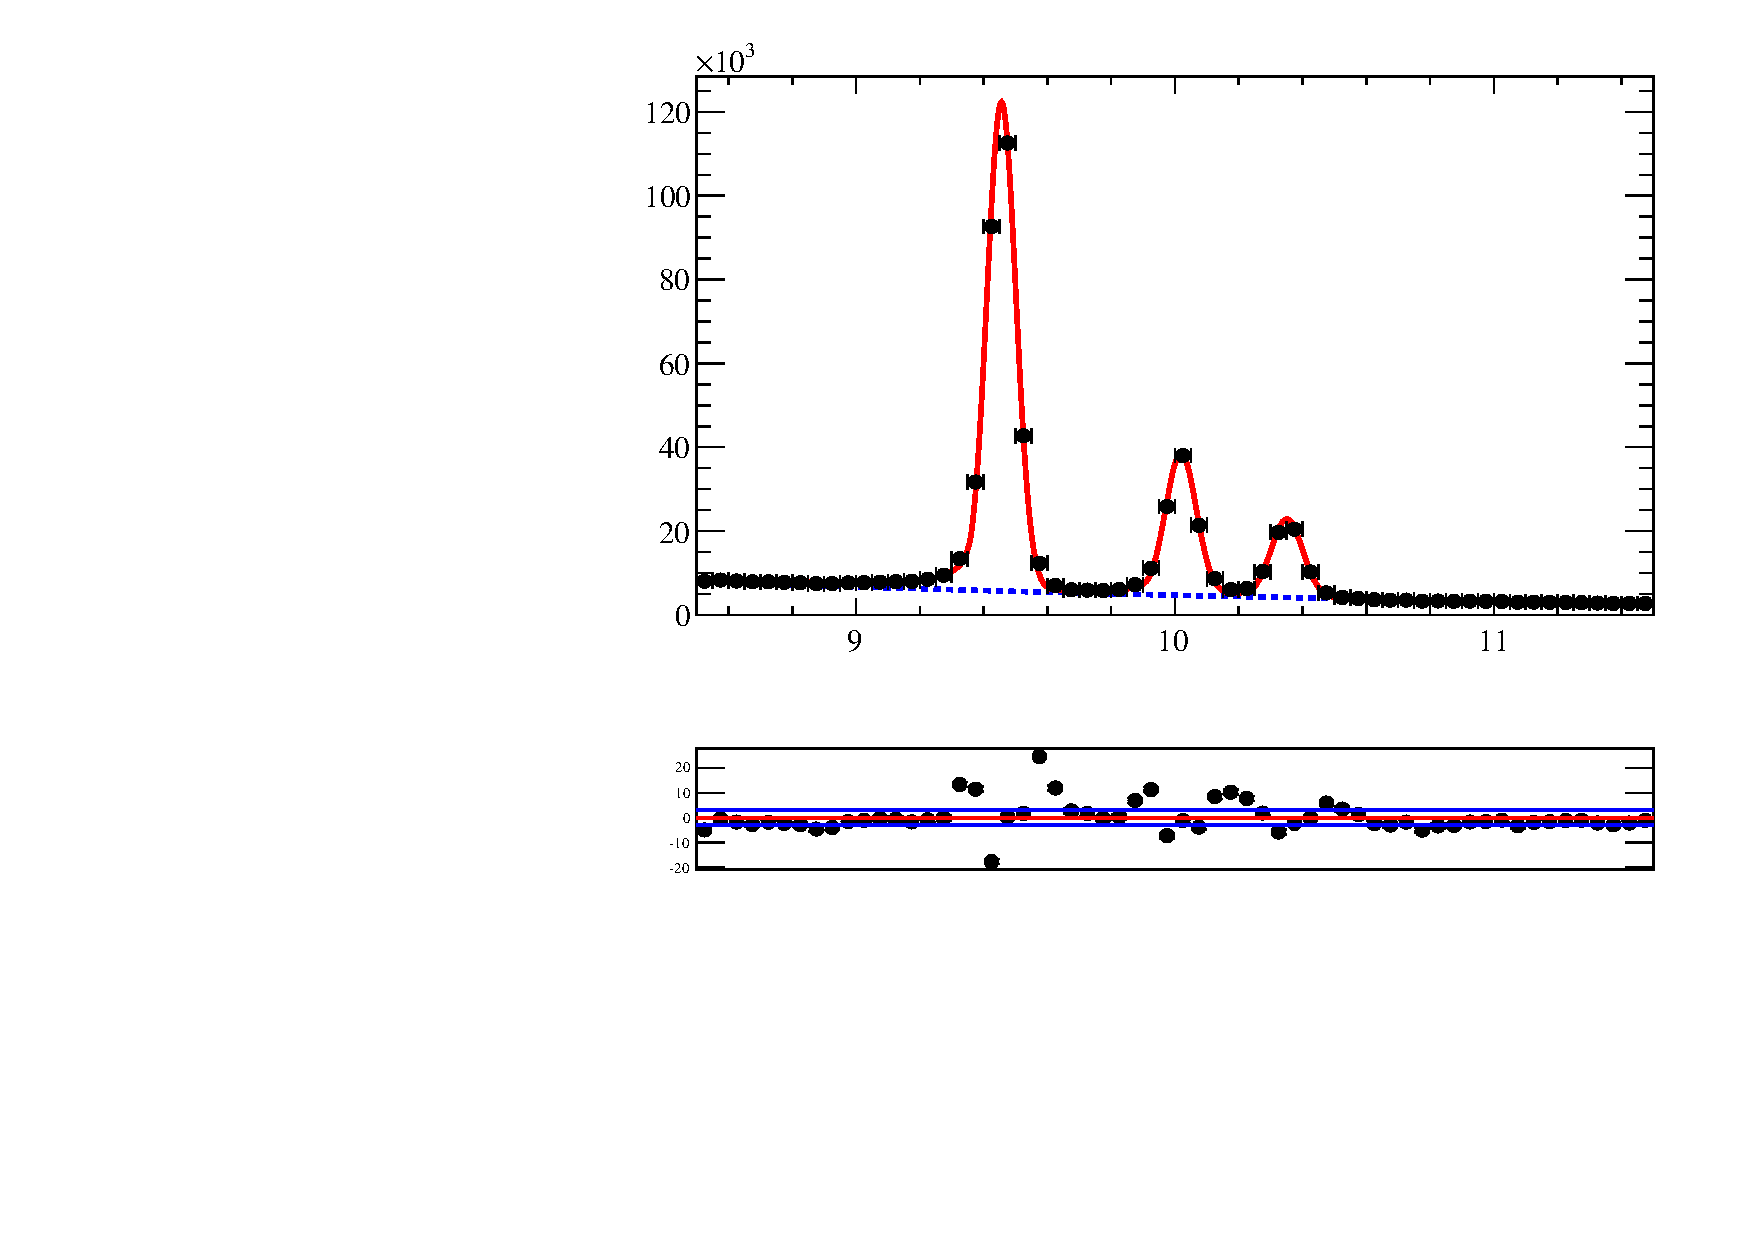
\includegraphics[width=75mm, height=60mm]{upsilon-fit/f2011_6_40}
    }
    \put(2,18){\small \begin{sideways}Candidates/(40\mevcc)\end{sideways}}
    \put(25, 13){$m_{\mumu} \left[\gevcc\right]$}
    \put(45,45){\sqs = 7 \tev}
    \put(35,38){$6 < p_T^{\mumu} < 40 \gevc$}
    % \graphpaper[5](0,0)(150, 60)
  \end{picture}
}
\begin{itemize}
\item 3 Crystal Ball functions for signal yields ($\alpha=2$, $n=5$).
\item Exponential function for combinatorial background.
\end{itemize}

\column{.5\textwidth}
\scalebox{0.5}{
    \begin{tabular}{lrrr}\toprule
    & \multicolumn{ 3 }{c}{$\mumu$ transverse momentum intervals (\gevc)} \\
     & & \multicolumn{2}{c}{6 --- 40} \\
    \cmidrule{3-4}
     && \sqs = 7 \tev & \sqs = 8\tev \\
    \midrule
    $N_{\Y1S}$ &&284,300 $\pm$ 600&661,800 $\pm$ 900 \\
    $N_{\Y2S}$ &&88,100 $\pm$ 400&204,800 $\pm$ 500 \\
    $N_{\Y3S}$ &&50,850 $\pm$ 290&116,700 $\pm$ 400 \\

    \rule{0pt}{4ex}$B$ &&294,300 $\pm$ 700&716,100 $\pm$ 1100 \\

    \rule{0pt}{4ex}$\mu_{\Y1S}, \mevcc$ &&9456.64 $\pm$ 0.09&9455.24 $\pm$ 0.06 \\
    % $\Delta m_{\Y2S}, \mevcc$ &&563.0&563.0 \\
    % $\Delta m_{\Y3S}, \mevcc$ &&894.9&894.9 \\

    \rule{0pt}{4ex}$\sigma_{\Y1S}, \mevcc$ &&45.23 $\pm$ 0.08&45.38 $\pm$ 0.06 \\

    % \rule{0pt}{4ex}$\alpha$ &&2.0&2.0 \\
    % $n$ &&1.0&1.0 \\

    % \rule{0pt}{4ex}$\tau$ &&-0.3574 $\pm$ 0.0023&-0.3526 $\pm$ 0.0015 \\

    % \rule{0pt}{4ex}$\chi^2/ndf$ &&24.9&49.5 \\    
    \bottomrule
    \end{tabular}   
}

\bigskip

\begin{itemize}
\item \Y1S mass is about 5 \mevcc lower than PDG value $9460.30 \pm  0.26$ \mevcc
\item In this study \OneS mass was fixed to $9.456 \gevcc$ 
\end{itemize}
\end{columns}


\end{frame}

